\section{Shared proxy-metric geometry and donor residuals}
\label{sec:target-geometry}

The additive experiment leaves two methodological questions open: whether
residuals from models that exclude their query observations improve
correction fitting, and whether a supervised input metric improves KAHM
forecasts. We study these factors with a raw ridge baseline and equally
trained geometric controls. The protocol, input roster, implementation,
and numerical dependencies were archived before full evaluation. The
design uses earlier findings but evaluates additional simulation draws
and four additional source collections.

\subsection{Baseline, residual targets, and matched procedures}
\label{sec:target-procedures}

The base $f_0$ is a raw-history ridge predictor, with its penalty selected
on a separate validation segment. Four gates use the same partition and
reference-selection rules: KAHM reconstruction, affine reconstruction,
locality-aware affine, and a center-distance RBF gate. All retain the
affinity-gated principal coordinates of Equation~\eqref{c:eq:local}.
The RBF-local control therefore describes local affine experts; it is
distinct from the raw Nystr\"om predictor. Requested banks contain
$2,4,8$ groups, rank two, at most 24 references per group and 512 fitting
histories. KAHM queries use the log-shifted Gaussian evaluation in
Section~\ref{c:sec:numerical}.

For each gate we fit three procedures: an identity metric with in-sample
residuals, an identity metric with out-of-fold (OOF) donor residuals, and a
learned metric with those same OOF residuals. The geometry is fitted on the training histories, subject to the
512-history cap. All three correction heads use exactly the same eligible rows,
so the natural-data OOF procedure does not gain a different correction
sample simply by excluding its initial donor prefix. For gate family $g$, let $\Gamma_g(x)$ denote its local feature
vector and let $q_g$ be the fitted residual correction, including
column standardization and a ridge readout. Its output has $H$
coordinates, one for each forecast offset. The forecast is
\[
 \widehat f_g(x)=f_0(x)+\gamma q_g\bigl(\Gamma_g(x)\bigr),
 \qquad \gamma\in\{0,\tfrac14,\tfrac12,1\}.
\]
The baseline and correction penalties use the same seven-value grid
$\{10^{-4},10^{-3},10^{-2},10^{-1},1,10,100\}$. The base is selected
first and held fixed. The candidate set contains zero correction and 21 positive
penalty--weight combinations. Validation chooses a nonzero correction
only when its error is strictly smaller than the baseline error;
subsequent ties retain the earlier candidate in the fixed grid order. The synthetic and archive evaluations retain their selected training-only fits,
without a pretest refit. The zero correction makes the baseline available during selection,
but validation selection does not guarantee improved test error.

Synthetic donors exclude complete independent episodes in four folds.
Natural-series donors use three forward blocks following an initial 40\%
of training origins; every donor target must have been available at the
first forecast origin of its query block. A donor selects its own ridge
penalty using an inner split of its own available data. The final base's
outer-validation choice never feeds backward into donor fitting.
Appendix~\ref{app:target-protocol} gives the boundary and small-sample
rules. Episode exclusion exploits independent synthetic trajectories, whereas
the forward-block construction respects target availability within a
natural series. The appropriate cross-validation design depends on
the forecasting assumptions \citep{Bergmeir2018CV}.

\paragraph{Residuals from different baselines.}
Condition on the fitted representation $\Gamma$, final baseline
$f_0$, and donor baseline $f_d$. Let $(X,Y)$ be a fresh evaluation
pair with $Y\in\R^H$, and write $Z=\Gamma(X)$. All expectations
in this paragraph refer to that evaluation distribution. Define
\[
 m_0(Z)=\E[Y-f_0(X)\mid Z],\qquad
 b_d(Z)=\E[f_0(X)-f_d(X)\mid Z].
\]
The correction minimizing the donor's population residual risk is
$q_d(Z)=m_0(Z)+b_d(Z)$. Assuming $Y$, $f_0(X)$, and $f_d(X)$ have
finite second moments, define $R_H(f)=H^{-1}\E\|Y-f(X)\|_2^2$. Then
\begin{equation}
 R_H(f_0)-R_H(f_0+q_d\circ\Gamma)
 =\frac1H\E\|m_0(Z)\|_2^2-\frac1H\E\|b_d(Z)\|_2^2.
 \label{eq:target-donor-transport}
\end{equation}
This elementary projection identity, proved with its fitted-correction
extension in Appendix~\ref{app:target-transport}, explains why donor
exclusion alone does not establish improvement of a different final
predictor. Chronological folds need not share the same distribution. Our recorded
donor/final disagreement on correction-training rows is a descriptive
diagnostic, not an estimate of either oracle term in
Equation~\eqref{eq:target-donor-transport}.

\subsection{A residual-supervised metric shared across geometries}
\label{sec:target-metric}

We learn a positive diagonal input metric through a Gaussian
kernel-regression proxy, following the supervised metric-learning
principle of \citet{Weinberger2007Metric}. Let $z_i\in\R^d$ denote a training-standardized history, with
$d=L$ equal to the history length, and let $s_i\in\R^H$ denote its donor residual vector,
centered by output and divided by one pooled residual standard deviation.
The shared scalar division preserves relative original-unit horizon
weights. On at most 256 training correction rows, set
\begin{align}
 d_\theta^2(z_i,z_j)&=\sum_{k=1}^{d}e^{\theta_k}(z_{ik}-z_{jk})^2,
 &p_{ij}(\theta)&=
 \frac{\exp\{-d_\theta^2(z_i,z_j)/(2\sigma^2)\}}
      {\sum_{l\in\mathcal A_i}\exp\{-d_\theta^2(z_i,z_l)/(2\sigma^2)\}},
 \quad j\in\mathcal A_i,\label{eq:target-metric-weights}\\
 \mathcal J(\eta)&=
 \frac{1}{|\mathcal I|H}\sum_{i\in\mathcal I}
 \left\|s_i-\sum_{j\in\mathcal A_i}p_{ij}(\theta)s_j\right\|_2^2
 +\frac{0.05}{d}\|\theta\|_2^2,
 &\theta&=\eta-\overline\eta\mathbf1.
 \label{eq:target-metric-objective}
\end{align}
The admissible donor-index set $\mathcal A_i$ excludes the query's episode for synthetic
data, or origins separated from the query by at most $L+H$ steps for natural
data. The set $\mathcal I$ contains queries with at least one admissible
donor. The vector $\eta\in\R^d$ contains free optimization parameters,
$\overline\eta=d^{-1}\sum_k\eta_k$, and $\theta$ is its centered
version. Thus $e^{\theta_k}$ is the metric weight of input coordinate $k$. The bandwidth $\sigma^2$ is the identity-metric
median positive admissible squared distance and remains fixed during
optimization. The box $|\eta_k|\leq\log(16)/2$ bounds the ratio between
the largest and smallest metric weights by 16; their geometric mean is
one. Indeed, $\theta_k-\theta_l=\eta_k-\eta_l$ is at most
$\log16$, and $\sum_k\theta_k=0$. The box constraint applies
to $\eta$; the centered coordinates $\theta_k$ need not lie in
the same interval.

The limited-memory bound-constrained quasi-Newton optimizer L-BFGS-B
uses the analytic gradient and at most 40 iterations.
Identity is the declared fallback for an unavailable or nonfinite
objective, constant residuals, or a worse final iterate. Finite improved
iterates at the iteration limit are retained with their convergence
status. No validation or test outcomes enter this optimization. Natural
metric donors may be earlier or later within the training period: this
is offline supervised fitting, separate from the forward construction
of baseline residuals.

The same learned weights are applied \emph{after} input standardization
for all four geometric gates; subsequent partitioning and local models
are refitted under that metric. This is a supervised kernel proxy
transferred to KAHM and its controls, not end-to-end minimization of
KAHM forecasting loss. Its training objective may decrease without
improving the final decoder. The comparison with equally trained local
controls tests whether any benefit is specific to the KAHM reconstruction.

\subsection{Declared evaluation and complete accounting}
\label{sec:target-evaluation}

Twelve independent repetitions of each of the nonlinear AR, Van der
Pol, and Duffing laws give 36 synthetic tasks. Each uses 128 training,
64 validation and 128 test episodes, history 12, direct offsets $1,4,12$
and the observation models in Appendix~\ref{c:app:methods}. Six prespecified comparisons per
law isolate learned-OOF KAHM versus ridge, learned versus identity
metric for OOF KAHM, OOF versus in-sample targets at the identity metric,
and learned-OOF KAHM versus each of the three equally trained geometric
controls. All 18 comparisons receive two-sided Bonferroni-adjusted
paired Student intervals over the 12 complete repetition differences.
Their coverage uses a normal approximation; origins and horizons do not
increase the replication count. These fresh simulations supply new
stochastic evidence on known laws, not new-domain confirmation.

Four additional Monash collections \citep{Godahewa2021Monash} provide
Australian state electricity demand, Bitcoin activity indicators,
Melbourne pedestrian counts, and KDD2018 air quality. Three series per
collection are selected using training-prefix eligibility and fixed hash ordering. The 12-series roster and split rules are specified in
Appendix~\ref{app:target-protocol}. These collections were not used in the earlier evaluations, although
some application domains overlap. They are not a
random sample of future forecasting applications. Natural results use
equal weights for series within source and for the four sources;
overlapping windows do not create independent source replications.

The 16 procedures comprise the 12 geometric corrections, ridge,
raw Nystr\"om-plus-linear regression, naive prediction, and a jointly
fitted raw-plus-KAHM ridge readout. The last is a secondary architecture
control and differs from the earlier concatenated Nystr\"om procedure.
The protocol reduces group counts when local training histories are
insufficiently distinct and uses predefined ridge fallbacks for
unavailable correction fits. Fewer than eight eligible correction rows
or a failed secondary joint head invokes a fallback for the affected
arms while retaining the available baselines. These fallback rules belong to this experiment; the additive study in
Section~\ref{sec:utility-extension} used a different failure policy.
Full-roster results remain unavailable if a primary baseline or required
task output is missing.

Warm pipeline cost charges each method for its complete required
baseline, donor, metric, bank, head-selection and serialization work,
including rejected candidates and fallbacks. Shared components are
charged once per standalone procedure. These are measured component
sums on one host, not repeated end-to-end deployment timings or minimum
possible complexity. Tables~\ref{tab:target-synthetic-main}
and~\ref{tab:target-archive-main} report the declared comparisons;
Appendix~\ref{app:target-results} retains all contrasts, source-level
results, fitting diagnostics, and resource records.

\subsection{Results: predictive gains and their attribution}
\label{sec:target-results}

All 48 tasks and 768 method--task forecast outputs completed, without
fallbacks. Learned-OOF KAHM reduces mean synthetic MSE relative to ridge
by 11.18\% on nonlinear AR, 53.26\% on Van der Pol, and 19.44\% on
Duffing. All three adjusted paired intervals favor the correction.
However, the three learned-versus-identity metric intervals and the
three OOF-versus-in-sample target intervals all include zero. These
comparisons do not establish equivalence; they leave the incremental
benefits of the two proposed changes unresolved at the declared
precision. Among nine comparisons with equally trained geometric
controls, none favors KAHM with an interval excluding zero. Five favor
the control: locality and RBF-local on Van der Pol, and all three on
Duffing. The other four remain unresolved. Thus the 18-contrast family
contains three favorable, five unfavorable, and ten unresolved results
for its designated candidates
(Appendix~\ref{app:target-results}). The secondary raw RBF predictor
also has lower mean MSE than learned-OOF KAHM on every law; this mean
ranking has no additional confirmatory interval.

On the four archive collections, learned-OOF KAHM has
source-balanced scaled MSE 1.272128 versus ridge's 1.300458, a
descriptive 2.18\% reduction. Its charged mean pipeline time is
0.1622\,s versus 0.001299\,s for ridge, or $124.9\times$ on this host.
The identity-metric in-sample KAHM procedure achieves a lower loss,
1.264589 (2.76\% below ridge), at $39.3\times$ ridge's time. The
lowest archive mean among the specified procedures is 1.257888 for identity-metric,
in-sample RBF-local correction. Learned-OOF affine and locality also
have lower means than learned-OOF KAHM, at 1.268679 and 1.266922,
respectively. Figure~\ref{fig:target-accuracy-cost} places the modest
archive accuracy changes alongside their measured computational cost;
the added metric stage is not supported as a default improvement by
these results.

Learned-OOF KAHM improves the mean in each of the four collections,
but improves only seven of the 12 individual series, worsens four,
and exactly retains ridge on one through zero correction. Omitting
each collection in turn leaves descriptive aggregate gains of
1.49--3.35\%. This sensitivity check shows that the sign does not
depend on retaining any one collection; it does not expand the
population represented by four selected collections or supply an
independent replication. These results establish improvement
over the selected ridge reference in the stated settings while
leaving a KAHM-specific advantage unsupported. The gains over ridge can also be obtained by simpler geometric
controls under these settings.

% Generated only from audited target-geometry predictions; no fitting.
\begin{table}[!htbp]
\centering\small\setlength{\tabcolsep}{4pt}
\caption{Fresh synthetic repetitions: mean test MSE $\times10^3$ over all 12 independent repetitions per law, with equal episode, origin and horizon weights. Every declared procedure is shown. A dash denotes an incomplete full roster; baseline fallbacks retain their actual forecasts. Differences are assessed by the 18 prespecified paired intervals in Table~\ref{tab:target-synthetic-intervals}, not by ranking these means.}
\label{tab:target-synthetic-main}
\begin{tabular}{lrrr}
\toprule
Procedure & Nonlinear AR & Van der Pol & Duffing \\
\midrule
Raw ridge & 5.057 & 44.140 & 6.916 \\
Raw RBF & 4.442 & 8.316 & 4.172 \\
Persistence / seasonal naive & 8.549 & 293.407 & 37.977 \\
Joint raw + KAHM & 4.465 & 17.009 & 5.277 \\
Fixed, IS KAHM & 4.478 & 21.380 & 5.468 \\
Fixed, IS Affine & 4.470 & 18.986 & 4.706 \\
Fixed, IS Locality & 4.503 & 13.699 & 4.508 \\
Fixed, IS RBF local & 4.427 & 15.987 & 5.318 \\
Fixed, OOF KAHM & 4.481 & 21.383 & 5.469 \\
Fixed, OOF Affine & 4.473 & 18.983 & 4.721 \\
Fixed, OOF Locality & 4.506 & 13.700 & 4.512 \\
Fixed, OOF RBF local & 4.431 & 15.988 & 5.321 \\
Learned, OOF KAHM & 4.492 & 20.629 & 5.572 \\
Learned, OOF Affine & 4.460 & 18.879 & 4.736 \\
Learned, OOF Locality & 4.530 & 13.968 & 4.536 \\
Learned, OOF RBF local & 4.408 & 15.460 & 5.328 \\
\bottomrule
\end{tabular}
\end{table}

% Generated only from audited target-geometry predictions; no fitting.
\begin{table}[!htbp]
\centering\small\setlength{\tabcolsep}{4pt}
\caption{Natural-data forecasting results: equal-collection means of equal-series scaled MSE and charged standalone wall seconds, covering four collections and three series per collection. Scaling uses training-only seasonal-difference MSE (first-difference fallback). IS denotes in-sample residuals and OOF denotes out-of-fold residuals. Change is relative to raw ridge; negative is favorable. Fallbacks predict raw ridge and retain attempted computation. Missing tasks make the affected full-roster means undefined. These are descriptive results, with no population confidence intervals or independence claims for adjacent origins.}
\label{tab:target-archive-main}
\begin{tabular}{lrrrrr}
\toprule
Procedure & Outputs & Scaled MSE & Change (\%) & Seconds & Fallbacks \\
\midrule
Raw ridge & 12/12 & 1.3005 & 0.00 & 0.001 & 0 \\
Raw RBF & 12/12 & 1.9483 & 49.82 & 0.005 & 0 \\
Persistence / seasonal naive & 12/12 & 1.8476 & 42.07 & 0.004 & 0 \\
Joint raw + KAHM & 12/12 & 1.4530 & 11.73 & 0.058 & 0 \\
Fixed, IS KAHM & 12/12 & 1.2646 & -2.76 & 0.051 & 0 \\
Fixed, IS Affine & 12/12 & 1.2584 & -3.24 & 0.029 & 0 \\
Fixed, IS Locality & 12/12 & 1.2635 & -2.84 & 0.028 & 0 \\
Fixed, IS RBF local & 12/12 & 1.2579 & -3.27 & 0.027 & 0 \\
Fixed, OOF KAHM & 12/12 & 1.2767 & -1.83 & 0.056 & 0 \\
Fixed, OOF Affine & 12/12 & 1.2731 & -2.11 & 0.034 & 0 \\
Fixed, OOF Locality & 12/12 & 1.2735 & -2.07 & 0.032 & 0 \\
Fixed, OOF RBF local & 12/12 & 1.2746 & -1.99 & 0.031 & 0 \\
Learned, OOF KAHM & 12/12 & 1.2721 & -2.18 & 0.162 & 0 \\
Learned, OOF Affine & 12/12 & 1.2687 & -2.44 & 0.142 & 0 \\
Learned, OOF Locality & 12/12 & 1.2669 & -2.58 & 0.141 & 0 \\
Learned, OOF RBF local & 12/12 & 1.2848 & -1.20 & 0.139 & 0 \\
\bottomrule
\end{tabular}
\end{table}

\begin{figure}[!htbp]
\centering
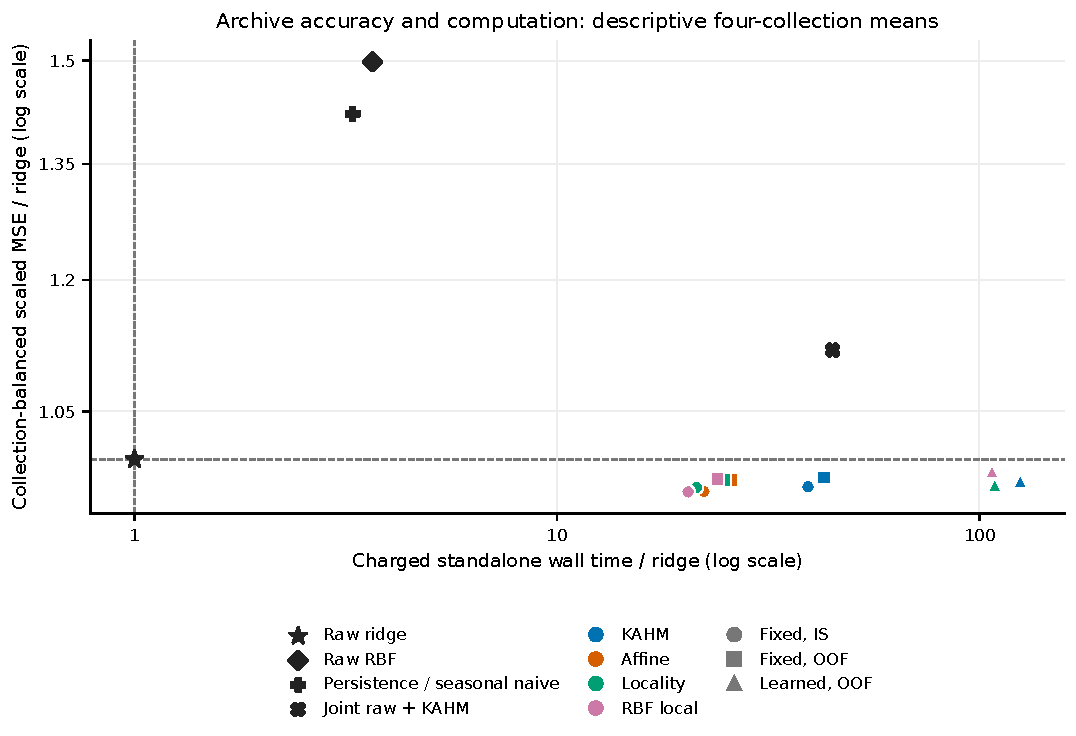
\includegraphics[width=0.96\linewidth]{generated/target_geometry/archive_accuracy_cost.pdf}
\caption{Accuracy and charged computation on the four archive
collections. Both axes divide the source-balanced method mean by the
corresponding ridge mean and use logarithmic scales. Lower loss and
lower time are preferable. Circles, squares, and triangles distinguish
identity/in-sample, identity/OOF, and learned/OOF procedures. Times
charge the complete required components of each method, including
selection; they are descriptive measurements from one host. The plot
shows all 16 procedures without implying uncertainty intervals or a
population-wide ranking.}
\label{fig:target-accuracy-cost}
\end{figure}
\FloatBarrier
